\chapter{Estado del arte}

\section{Marco teórico}
Los seres humanos cuando hablan entre ellos suelen usar términos más efímeros para trabajar con la realidad, y es que, muchas veces trabajar con cantidad de cuantitativas no es intuitivo para la mente. \\ \\
De esta vagueza del lenguaje, en 1965, Lofti A. Zadeh publicó lo que hoy se conoce como teoría de conjuntos difusos. La teoría de conjuntos difusas funciona utilizando la idea que subyace detrás de la función característica de los conjuntos clásicos, que se define de la siguiente forma: \\ \\
Sea $A$ un conjunto cualesquiera, se define la función característica $\chi_A(x)$ de $A$ como:
\[
	\chi_A(x) = \left\{
		\begin{array}{ccc}
			1 & si & x \in A \\
			0 & si & x \notin A
		\end{array}
	\right.
\]

Por otro lado, para definir lo que es un conjunto difuso se generaliza la idea de función característica a una función que toma valores en $[0, 1]$, que se puede definir como sigue, un conjunto difuso $B$ se define como un par ordenado dado, por $(\mu_B, \mathbb{U})$ donde $\mu_B : \mathbb{U} \longrightarrow [0,1]$ y $\mathbb{U}$ es el conjunto de discurso. \hyperref[def:subconjunto_difuso]{(Subconjunto difuso)} \\ \\
Dentro de la teoría de conjuntos difusos también se pueden desarrollar una serie de términos para tratar de definir lo que es un número difuso, se puede encontrar más información \hyperref[def:numero_difuso]{aquí}, pero básicamente cuando se habla de número difuso es un conjunto difuso que cumple una serie de condiciones de regularidad, un ejemplo clásico de número difuso corresponde a los números triangulares:
\begin{figure}[H]
	\centering
	\frame{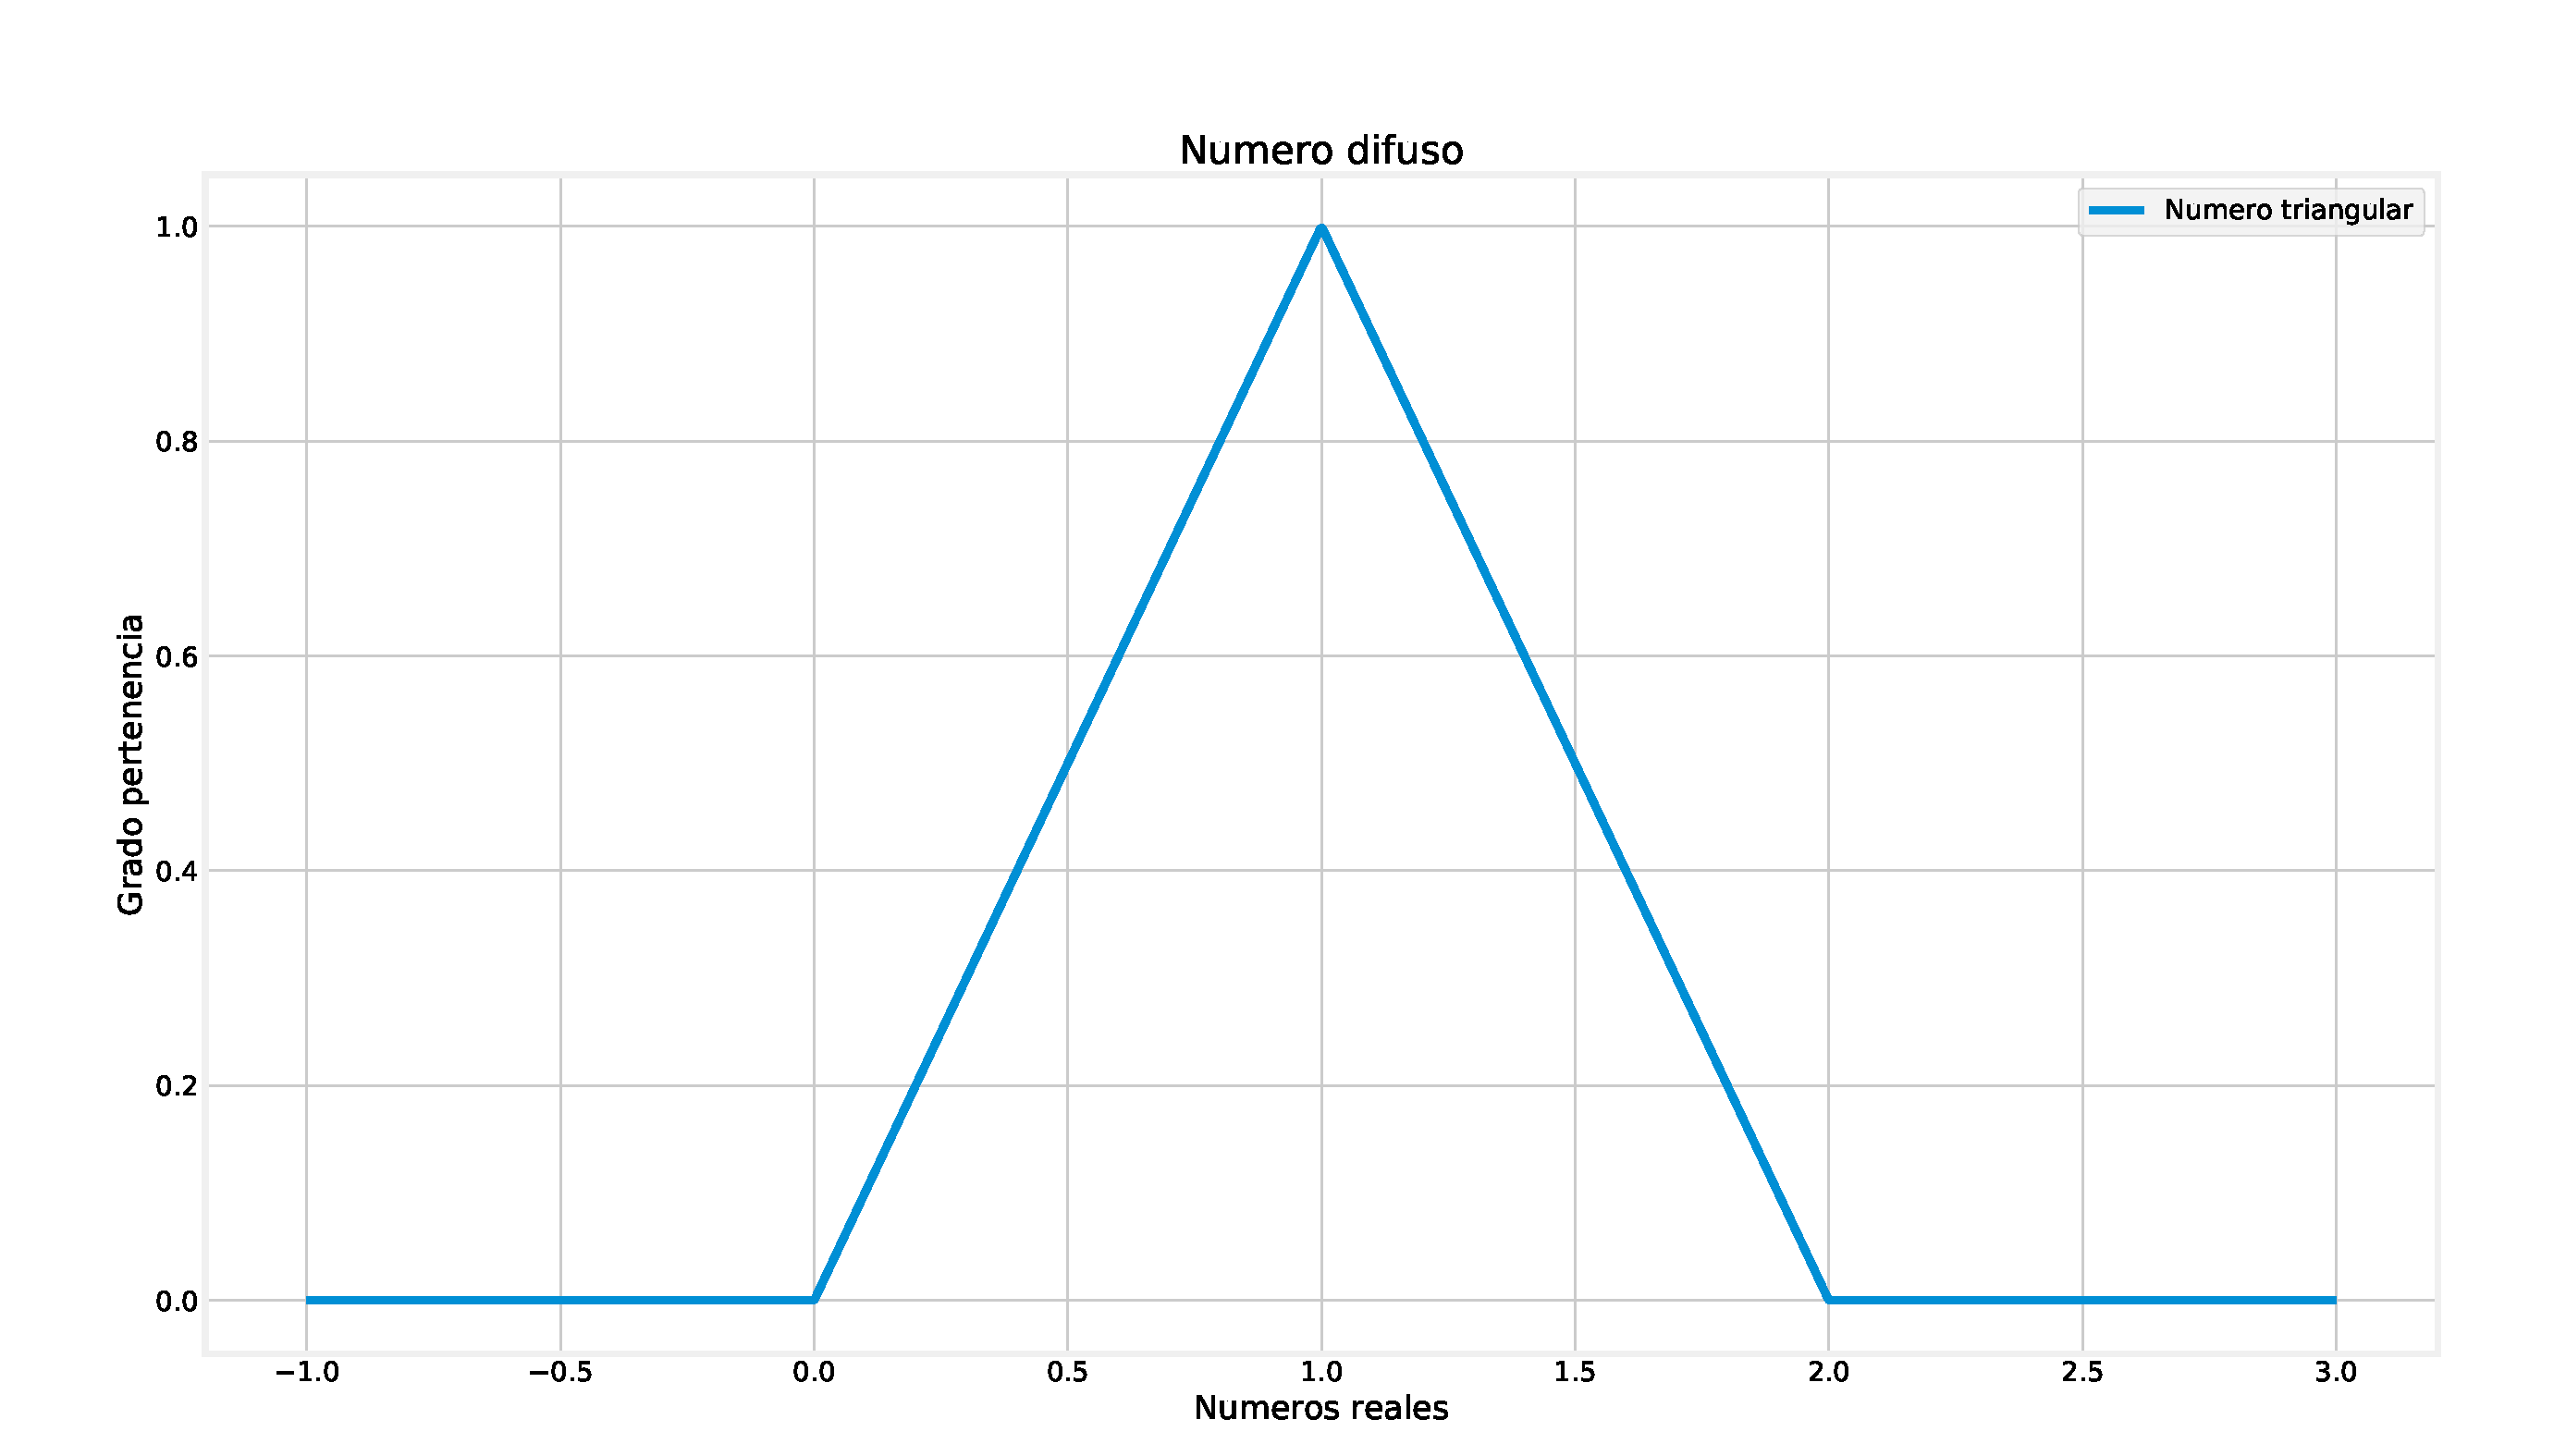
\includegraphics[width=\textwidth]{grafica_triangular}}
	\caption{Ejemplo de número triangular}
\end{figure}
Por otro lado como ocurren en los números ordinarios, también se le pueden asociar operaciones aritméticas básicas como la suma, el producto, la resta y la división. Las definiciones de suma, producto y división de números difusos funciona de forma bastante intuitiva, sin embargo, definir el concepto de resta de dos números difusos es más complejo, pero que nos permitirá hacer derivadas de funciones difusas, que es uno de los objetivos.
\\ \\
Otro concepto interesante, a tener en cuenta y que marcó una revolución es la introducción del \hyperref[def:zadeh]{principio de extensión de Zadeh}, que nos permite obtener una función difusa mediante un conjunto difuso y una función clásica. Todos estos conceptos introducidos por Lofti A. Zadeh da lugar a un marco teórico que permite desarrollar conceptos clásicos del análisis.

\section{Objeto de este estudio}
En este trabajo se busca generalizar el concepto de ecuación diferencial a un marco difuso, esto tiene todo el sentido del mundo pues la realidad siempre se nos presenta de esta forma. A lo largo del siglo $XX$ esto se vio reflejado también no sólo en las matemáticas, sino que otras ciencias como la química se vieron afectadas por la incertidumbre, que empezó a hacerse hueco después del principio de incertidumbre de Heissenberg. Así como en la física, existen siempre errores en las medidas y el problema de no existir medidas con precisión infinita. \\ \\
Todas estas cantidades que no son exactas, sino que oscilan entre ciertos valores se pueden representar como números difusos, y es aquí donde florece el potencial brutal de las ecuaciones diferenciales difusas. \\ \\
Por ejemplo, los instrumentos de medidas de un avión en condiciones extremas puede que no sean tan precisos como esperamos, pero si conocemos el error que se comete, no nos importa, pues podemos expresar las medidas como números difusos y resolver trayectorias planteando ecuaciones diferenciales difusas. \\
Las constantes clásicas de la física tampoco están exentas de errores, podemos obtener resultados más fidedignos si planteamos las ecuaciones a través de números difusos. \\ \\
